\section{Exercise 6}

Consider the following code: 
\begin{verbnobox}[\verbarg]
#include <stdio.h>

typedef struct 
{
    char buf2[15];
    char buf[64];
} data_t;
// This function writes 5 times 15 char in data.buf
int scramble(int *sequence) 
{
    data_t data;

    for (int i = 0; i < 5; i++)
    {
        scanf("\%15s", data.buf2);
        strncpy(&data.buf[sequence[i]*15], data.buf2, 15);
        printf(data.buf);
    }
}

void main() 
{
    int sequence[5] = {3,1,4,0,2};

    scramble(sequence);
}
\end{verbnobox}
The C standard library is loaded at a known address during every execution of the program, and that the address of the function system() is \texttt{0xf4d0e2d3}.
Environment variables are located in the highest addresses. 
The program is compiled for the x86 architecture (32 bit) and for an environment that adopts the usual cdecl calling convention. 
Furthermore, assume that no compiler-level or OS-level mitigation against exploiting memory corruption errors are present (unless specified otherwise).
\begin{enumerate}
    \item The program is affected by typical buffer overflow and format string vulnerabilities.
        Find them.
    \item Focus only on the stack-based buffer overflow(s) you found. 
        Write an exploit for this vulnerability that must execute the following shellcode, composed of 8 bytes, which opens a shell:
\begin{verbatim}
0x20 0x30 0x40 0x50 0x60 0x70 0x80 0x90
\end{verbatim}
        Describe all the steps and assumptions required for the successful exploitation of the vulnerability.
        Include also any assumption on how you must call and run the program: e.g., the values for the command-line arguments required to trigger the exploit correctly and/or environment variables, (if any), the input provided during the execution, if multiple executions are necessary.
        Make sure that you show how the exploit will appear in the process memory with respect to the stack layout right before and after the execution of the vulnerable line during the program exploitation showing:
        \begin{itemize}
            \item Direction of growth and high-low addresses;
            \item  The name of each allocated variable;
            \item  The content of relevant registers (i.e., EBP, ESP);
            \item  The functions stack frames.
        \end{itemize} 
        Show also the content of the caller frame.
    \item Write an exploit for this vulnerability that executes the previous shell code, assuming that you have already prepared the memory (the shell code has been positioned in a place under the control of the attacker) with the correct arguments. 
        Assume that: 
        \begin{itemize}
            \item The address of the return address (saved EIP) of the function exploited is: 0x8da0fee4 (i.e., where to write). 
            \item The address of the first instruction of the shell code is at 0xd3f4e2d0 (i.e., what to write). 
            \item The displacement on the stack of the vulnerable function's argument is: 7
        \end{itemize}
        Knowing that dec(0xd3f4) = 54260 and dec(0xe2d0)=58064, write the exploit clearly, describe all the steps, assumptions and the components of the format string required to successfully exploit the vulnerability. 
        Include also any assumption on how you must call and run the program: e.g., the values for the command-line arguments required to trigger the exploit correctly and/or environment variables (if any), the input provided during the execution.
    \item Assume now that the main function is modified as follows:
\begin{verbatim}
void main() 
{
    int sequence[5];
    srand(0); // seed the random number generator with seed=0

    for (int i = 0; i < 5; i++) {
        sequence[i] = rand() % 5; // generate a random number between 0 and 4
    }

    scramble(sequence);
}
\end{verbatim}
        Is any of the previous exploits working without any modification? 
        If yes explain why, if not motivate your answer and provide an alternative solution: describe all the steps and assumptions required for the successful exploitation of the vulnerability. 
        Include also any assumption on how you must call and run the program: e.g., the values for the command-line arguments required to trigger the exploit correctly and/or environment variables, (if any), the input provided during the execution, if multiple executions are necessary.
\end{enumerate}

\subsection*{Solution}
\begin{enumerate}
    \item The buffer overflow is at line sixteen because the sequence contains 4 that multiplied by 15 goes out of the memory allocated for buf. 
        The format string is at line seventeen because there is a printf of buf. 
    \item I can place the shell code in the environment variables, I get the address of the variable, and I use the address of the variable when exploiting the overflow. 
        Alternatively, I can also put directly the shell code in the stack. 
        The stack will be the following: 
        \begin{figure}[H]
            \centering
            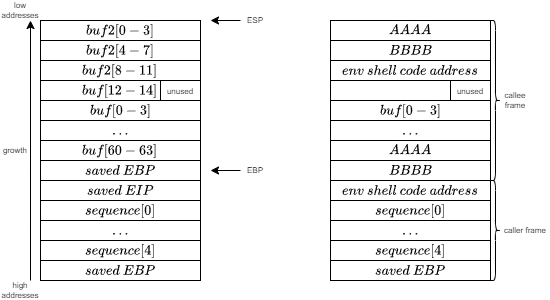
\includegraphics[width=0.75\linewidth]{images/stack9.png}
        \end{figure}
    \item The format string is composed as follows: 
        \begin{itemize}
            \item The address of the saved EIP + 2: /xe6/xfe/xa0/x8d
            \item The address of the saved EIP: /xe4/xfe/xa0/x8d
            \item The first argument to write is: 54260 - 8 = 54252
            \item The displacement is 7
            \item The second argument to write is the difference between the numbers: 58064 - 54260 = 3804.
        \end{itemize}
        The first number to write is 54260 since it is lower than 58064
        The final string is: 
\begin{verbatim}
/xe6/xfe/xa0/x8d/xe4/xfe/xa0/x8d%54252c%7$hn%3804c%8$hn
\end{verbatim}
        Due to the limitation of 15 characters for the first buffer this must be written in multiple steps of the cycle.
    \item The buffer overflow can be achieved, but we need to find a four in the sequence array. 
        However, the seed 0 for the srand function is problematic since it may not give a modulo five number. 
        Since it is fixed if at the first run the exploit does not work, it will not work since the sequence will be always the same. 
\end{enumerate}